%_________Einleitung__________________________________
\chapter{Modular Modeling of Underwater Robot Prototype}

Based \cite{opencv_library} on the ideas of the computational underwater robot design, the designer should be able to assemble a underwater robot from a collection of components (hull enclosure, batteries, fins, thrusters, CPU, IMU, sensor and so on). The customizable robot structure implies the robot dynamics is determined by number and type of constituent components and their geometric variables. Unlike the conventional modeling method for which all components are fixed, in this chapter, we model the robot modularly. More precisely, each robot component is approximated as simple geometric shape determined by several size parameters. Then we can parametrize the mass, the moment of inertia and the hydrodynamic coefficients with these parameters. In addition, the position and orientation parameters also contribute the dynamics of the whole robot. By means of this modeling approach, a customizable dynamic model is obtained.

The underwater vehicles are mainly composed of hull and actuators and actuators can be further divided into thrusters and control fins. The modular modeling method is mainly adapted from~\cite{Sia1999}. We only consider the hydrodynamic effects of hull, while the added mass and hydrodynamic damping of fins and thrusters are also calculated. Also, we ignore the moment of inertia of fins and thrusters and assume that it is merely determined by hull components. Besides, we take the electronic devices into account and model them as cuboid. They have contribution to the total mass and moment of inertia of the robot and specify the minimal size of the hull volume.   

The inertia tensor for each modular component $s$ with respect to its center of mass $CG_{s}$  is given by
\begin{align}
\emph{\textbf{I}}_{g,s}=
\begin{pmatrix}
I_{xx,s}&0&0\\
0&I_{yy,s}&0\\
0&0&I_{zz,s}
\end{pmatrix}.
\end{align} 

\section{Modeling of Hull Components}
As the main body of the underwater robot, the navigation system, sensory system and the power supply system are embedded in it. 

The hull shell is modeled as hollow cylinder, as illustrated in Figure ~\ref{fig:HullModeling}. We use three parameters to characterize it including the inner radius $r_{H,i}$, the outer radius $r_{H,o}$ and the hull length $l_{H}$. Then its mass and moment of inertia with respect to its center of gravity can be calculated as follows:   
\begin{figure}
\centering
\begin{tikzpicture}[x=1.5cm,y=1.5cm,>=latex']
	\coordinate (O) at (0,0) node[above] {\small ${CO}$};
	\draw[black,fill=black] (0,0) circle (.5ex);
	\draw (-1.55,-1.515) arc (-30:30:0.5);
	\draw (-1.55,-1.515) arc (-150:-210:0.5);
	\draw (-1.55,-1.515) arc (75:15:0.5);
	\draw (-1.55,-1.515) arc (195:255:0.5);
	\draw (-1.55,-1.515) arc (-15:-75:0.5);
	\draw (-1.55,-1.515) arc (105:165:0.5);
	\draw [->,blue,line width=0.65mm,] (-1.5,-1.5) (O) -- (-1.55,-1.515)node[midway,above] {\small $\vec{r}_{T}$};
    \draw [->,blue,line width=0.65mm,] (-2,-2) arc[x radius=0.75cm, y radius =.75cm, start angle=-150, end angle=-30]node[below right] {\small $\vec{b}_{T}$};
	\draw[black,fill=black] (-1.55,-1.55) circle (.4ex);
	\draw [->,blue,line width=0.65mm,](-1.55,-1.515) -- (-1,-1.55) node[right] {\small $\vec{d}_{T}$};
	\coordinate (OD) at(0,-1);
	% plot the x-axis
	\draw [dashed] (O) -- (2,0);
	\draw [dashed] (O) -- (0,-1);
	\draw [->](2,0) -- (3,0) node[right] {$x_{b}$};
	\draw [dashed] (O) -- (-2,0);
	\draw [->](0,-1) -- (0,-2) node[below right] {$z_{b}$};
	\draw (-2,0) circle(0.3 and 1);
	\draw (-2,0) circle(0.24 and 0.8);
	\draw [dashed](2,0) circle(0.24 and 0.8);
	\draw [dashed](0,0) circle(0.24 and 0.8);
	\draw [dashed] (2,1) arc[start angle=90,end angle=270,x radius=0.3,y radius=1];
	\draw [name path=P2] (2,1) arc[start angle=90,end angle=-90,x radius=0.3,y radius=1];
	\draw [dashed] (0,1) arc[start angle=90,end angle=270,x radius=0.3,y radius=1];
	\draw [name path=P] (0,1) arc[start angle=90,end angle=-90,x radius=0.3,y radius=1];
	\draw (-2,1)--(2,1);
	\draw (-2,-1)--(2,-1);
	\path [name path=PP] (O) -- (1,-1);
	\path [name intersections={of=P and PP}];
	\coordinate (X1) at (intersection-1);
	\draw[dashed] (O)--(X1);
	\draw [->](X1) -- (1.35,-1.35) node[below left] {$y_{b}$};
	\draw [<->] (-2,1.2) -- (2,1.2) node [midway, above] {$l_{H}$};
	\draw (-2,1.1)--(-2,1.4);
	\draw (2,1.1)--(2,1.4);
	% legend for the radius
	\draw (-2.1,1)--(-3.5,1);
	\draw (-2.1,0)--(-3.5,0);
	\draw (-2.1,0.8)--(-2.9,0.8);
    \draw [<->] (-3,0) -- (-3,1) node [midway, left] {$r_{H,o}$};
    \draw [<->] (-2.5,0) -- (-2.5,0.8) node [midway, left] {$r_{H,i}$};
	\end{tikzpicture}
\caption{Modeling of hull as hollow cylinder} \label{fig:HullModeling}
\end{figure}
\begin{align}
m_{H}=\rho_{H}\pi (r_{H,o}^{2}-r_{H,i}^{2})l_{H},
\end{align}
\begin{align}
I_{xx,H}=\dfrac{1}{2}m_{H}(r_{H,o}^{2}+r_{H,i}^{2}),
\end{align}
and
\begin{align}
I_{yy,H}=I_{zz,H}=\dfrac{1}{4}m_{H}(r_{H,o}^{2}+r_{H,i}^{2}+\dfrac{l_{H}^{2}}{3}).
\end{align}
In the following part, we simplify the notation of $r_{H,o}$ as $r_{H}$.
Within the hull, we model the battery as solid cylinder, based on the defined coordinate in \ref{fig:BatteryModeling}, the mass and moment of inertia are given as
\begin{align}
m_{bat}=\rho\pi r_{bat}^{2} l_{bat},
\end{align}
\begin{align}
I_{xx,bat}=I_{yy,bat}=\dfrac{1}{12}m_{bat}(3r_{bat}^{2}+l_{bat}^{2}),
\end{align}
and
\begin{align}
I_{zz,bat}=\dfrac{1}{2}m_{bat}r_{bat}^{2}
\end{align}
\begin{figure}
\centering
\begin{tikzpicture}[x=1.5cm,y=1.5cm,>=latex']
	\coordinate (O) at (0,0);
	\coordinate (OD) at(0,-1);
	\draw[dashed] (O) -- (1,0);
	\draw [->](1,0) -- (2,0) node[right] {$x$};
	\draw[dashed,-serif cm] (O) -- (0,-1);
	\draw[dashed,-serif cm] (O) -- (0,1);
	\draw [->](0,-1) -- (0,-2) node[below right] {$z$};
	\draw (0,1) circle(1 and 0.3);
	% \draw (0,-1) circle(1 and 0.3);
	\draw[dashed] (O) +(0:1) arc[start angle=0,end angle=180,x radius=1,y radius=0.3];
	\draw[name path=P] (O) +(0:1) arc[start angle=0,end angle=-180,x radius=1,y radius=0.3];
		\draw[dashed] (OD) +(0:1) arc[start angle=0,end angle=180,x radius=1,y radius=0.3];
	\draw[name path=PD] (OD) +(0:1) arc[start angle=0,end angle=-180,x radius=1,y radius=0.3];
	\draw (-1,-1)--(-1,1);
	\draw (1,-1)--(1,1);
	\path[name path=P1] (O) -- (-1,-1);
	\path [name intersections={of=P and P1}];
	\coordinate (X1) at (intersection-1);
	\draw[dashed] (O)--(X1);
	\draw [->](X1) -- (-1.35,-1.35) node[below left] {$y$};
	\draw [<->] (-1.2,1) -- (-1.2,-1) node [midway, left] {$l_{bat}$};
	\draw (-1,1.1)--(-1,1.4);
	\draw (0,1)--(0,1.4);
    \draw [<->] (-1,1.2) -- (0,1.2) node [midway, below] {$r_{bat}$};
    	\end{tikzpicture}
\caption{Modeling of battery as solid cylinder} \label{fig:BatteryModeling}
\end{figure}
All other devices are assumed to have a constant mass $m_{d}$ and a constant moment of inertia $\emph{\textbf{I}}_{d}$ with respect to the body frame.

\section{Modeling of Control Actuators}
Usually, fins and thrusters are used as actuators. In the second optimization phase, we want to optimize the geometric parameters of all actuators. For the design of robots, geometric placement of all  actuators plays an decisive role for controlling performance. To find an optimal geometric properties of actuators in the designing phase, appropriate models for actuators are required to estimate the generated control efforts under different actuator configurations, and the lift of fin is treated as the control input.  
 
\subsection{Modeling of Thrusters}
\label{Subsection:ModelingofThrusters}
For modeling of thrusters, we adopt the modeling methods from~\cite{Du2016}. 
Based on this modeling, each thruster is parameterized by the motor orientaion $\vec{d}_{T}$~(unit vector), the motor position $\vec{r}_{T}$ in the body frame $\lbrace b \rbrace$ and the motor spin direction  $b_{T}\in \lbrace-1,1\rbrace$. We use $u_{T}$ and $m_{T,r}$ to denote the magnitude of the thrust force and torque generated by the propeller rotation, respectively.

Yoerger et al.~(\cite{PropellerModel}) proposed the one-state model for the propeller.
The torque $Q_{m}$ and thrust $T$ has the following relationship:
\begin{align}
\dot{\omega}_{p}=\beta Q_{m}-\alpha\omega_{p}|\omega_{p}|
\label{EQ:PropellerDynamics1}
\end{align}
\begin{align}
T=C_{t}\omega_{p}|\omega_{p}|
\label{EQ:PropellerDynamics2}
\end{align}
where $\omega_{p}$ is the propeller angular velocity, $\alpha$ and $\beta$ are constant model parameters and $C_{t}$ is a proportionality constant. The three parameters $\alpha$, $\beta$ and $C_{t}$ require to be identified. 

%Within each trim trajectory segment, all desired inputs should be constant, thus %the spinning velocity should be time-invariant, 
%i.e. $\dot{\omega}_{p}=0$, 
If the propeller rotates at steady state, i.e. $\dot{\omega}_{p}=0$, then according to (\ref{EQ:PropellerDynamics1}) and (\ref{EQ:PropellerDynamics2}), the relationship between the thrust generated by the propeller and the rotation torque can be described with the following equation:
\begin{align}
Q_{m}=\dfrac{\alpha}{C_{t}\beta}T,
\end{align}
which means that the torque generated due to the rotation of propellers is proportional to the thrust force of the propeller. Thus, we can assume the torque $m_{T,r}$ is proportional to the thrust force $u_{T}$
\begin{align}
m_{T,r}=\lambda_{T} u_{T},
\end{align}   
where $\lambda_{T}$ is the torque-force ratio. Taking the thruster motor orientation and the spin direction into consideration, we can have the rotation torque vector as
\begin{align}
\vec{m}_{T,r}=b_{T}\lambda_{T} u_{T}\vec{d}_{T}.
\end{align} 
Additionally, the thrust force will produce the thrust torque $\vec{m}_{T,t}$. For calculation of thrust torque, the center of gravity is assumed to be located in the body frame origin $CO$. Then the thrust torque can be expressed as
\begin{align}
\vec{m}_{T,t}=\vec{r}_{T}\times u_{T}\vec{d}_{T},
\end{align}
where $\vec{r}_{T}=(x_{T}, y_{T}, z_{T})$ is the position vector of the thruster in the body frame $\lbrace b \rbrace$.
Combining the thrust torque and the rotation torque, we express the total torque produced by a thruster as 
\begin{align}
\vec{m}_{T}=\vec{m}_{T,r}+\vec{m}_{T,t}=b_{T}\lambda_{T} u_{T}\vec{d}_{T}+\vec{r}_{T}\times u_{T}\vec{d}_{T} \in \mathbb{R}^{3}
\end{align}

The force direction is determined by the thruster motor orientation $\vec{d}_{T}$ and the force vector $\vec{f}_{T}$ can be represented as
\begin{align}
\vec{f}_{T}=u_{T}\vec{d}_{T} \in \mathbb{R}^{3}
\end{align}
The generalised force vector for thruster is defined as
\begin{align}
\vec{\tau}_{T}=\begin{pmatrix}
\vec{f}_{T} \\ \vec{m}_{T}
\end{pmatrix}
\end{align} 
If we treat the thrust as the control input, we can define an unique mapping vector for a thruster based on its geometric parameters.
\begin{align}
\emph{\textbf{B}}_{T}=
\begin{pmatrix}
\vec{d}_{T} \\
b_{T}\lambda_{T} \vec{d}_{T}+\vec{r}_{T}\times \vec{d}_{T}
\end{pmatrix} \in \mathbb{R}^{6}. \label{EQ:ThrusterMappingVector}
\end{align}
Then the generalised force generated by thrust can be in the following form:
\begin{align}
\vec{\tau}_{T}=\emph{\textbf{B}}_{T}u_{T}
\end{align}
 
\subsection{Modeling of Control Fins}
An accurate hydrodynamic modeling of control fins in Appendix C introduces high order nonlinear terms into the input matrix $\emph{\textbf{B}}_{a}$. The velocity of fin middle point in the body frame $\lbrace b \rbrace$ is denoted by $\vec{v}_{fin}=(u_{fin},~v_{fin},~w_{fin})^{T}$ and its three components have the following relationship with the robot linear velocity $\vec{v}=(u,~v,~w)^{T}$: 
\begin{align}
u_{fin}=u+z_{fin}q-y_{fin}r,
\end{align}
\begin{align}
v_{fin}=v+x_{fin}r-z_{fin}p,
\end{align}
\begin{align}
w_{fin}=w+y_{fin}p-x_{fin}q.
\end{align}
Then the fin velocity $\vec{v}_{fin}^{f}=(u_{fin}^{f},~v_{fin}^{f},~w_{fin}^{f})^{T}$ in the fin frame $\lbrace f \rbrace$ is calculated as:
\begin{align}
\vec{v}_{fin}^{f}=\emph{\textbf{R}}_{b}^{f}\vec{v}_{fin},
\end{align}
where $\emph{\textbf{R}}_{b}^{f}$ is determined by the fin position vector $\vec{r}_{F}$ in the body frame $\lbrace f \rbrace$. Then the angle of attack $\alpha$ is calculated as
\begin{align}
\alpha=atan2(w_{fin}^{f},u_{fin}^{f}).
\end{align} 
The $atan2$ can not be approximated by a polynomial term numerically. Furthermore, the lift and drag coefficients $C_{L}$, $C_{D}$ are piecewise functions of the angle of attack $\alpha$. We are able to use high-order polynomials to approximate them. The lift coefficient characteristic curve is depicted in Figure~\ref{FIG:LiftCoefficient}. The curve fitting result is shown in Figure~\ref{FIG:LiftApprox} and the relationship between $C_{L}$ and the attack angle $\alpha$ is
\begin{align}
C_{L}=-0.1463\alpha^{8}+1.234\alpha^{6}-3.61\alpha^{2}+0.09403.
\end{align}
Similarly, we are able to approximate the drag coefficient characteristic curve in~\ref{FIG:DragCoefficient} with high-order polynomials whose result is depicted in Figure~\ref{FIG:DragApprox}. The fitting function is:
\begin{align}
C_{D}=-0.4653\alpha^{9}-3.219\alpha^{7}+8.356\alpha^{5}-9.75\alpha^{3}+3.729\alpha.
\end{align}
These two high-order terms require considerably large computational capacity for the optimization. The aforementioned two problems from accurate hydrodynamic modeling make the optimization problem nearly unsolvable.

\begin{figure}
\centering
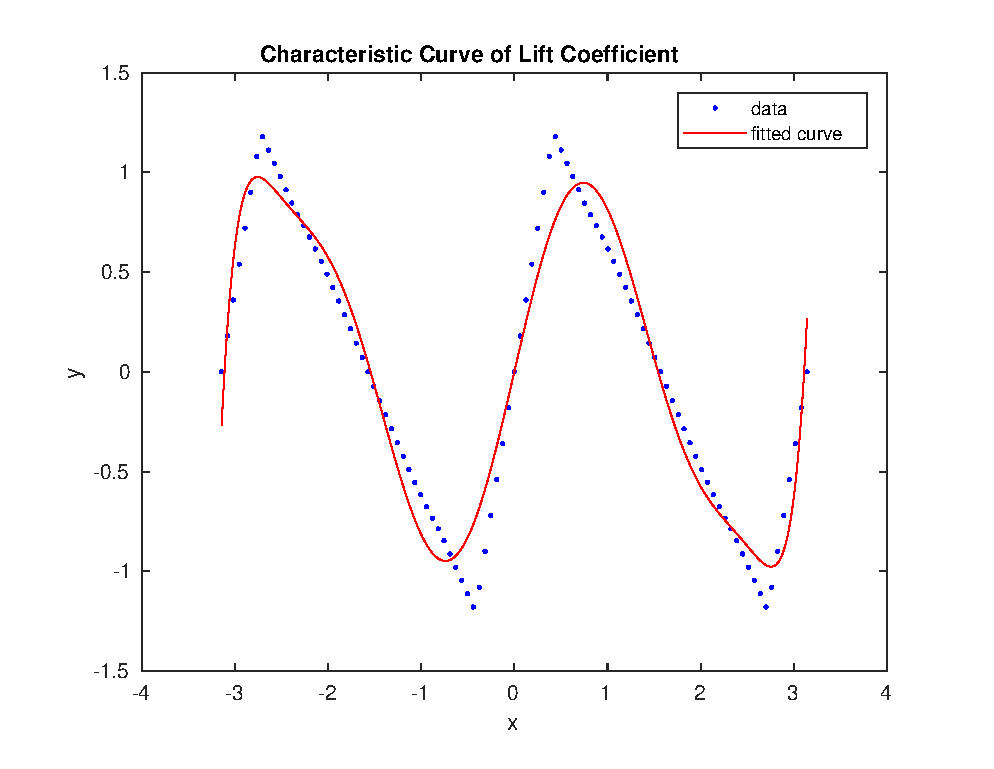
\includegraphics[width=0.75\textwidth]{liftappro.eps}
\caption{Approximation of relationship between lift coefficient $C_{L}$ and attack angle $\alpha$}	
\label{FIG:LiftApprox}
\end{figure}
\begin{figure}
\centering
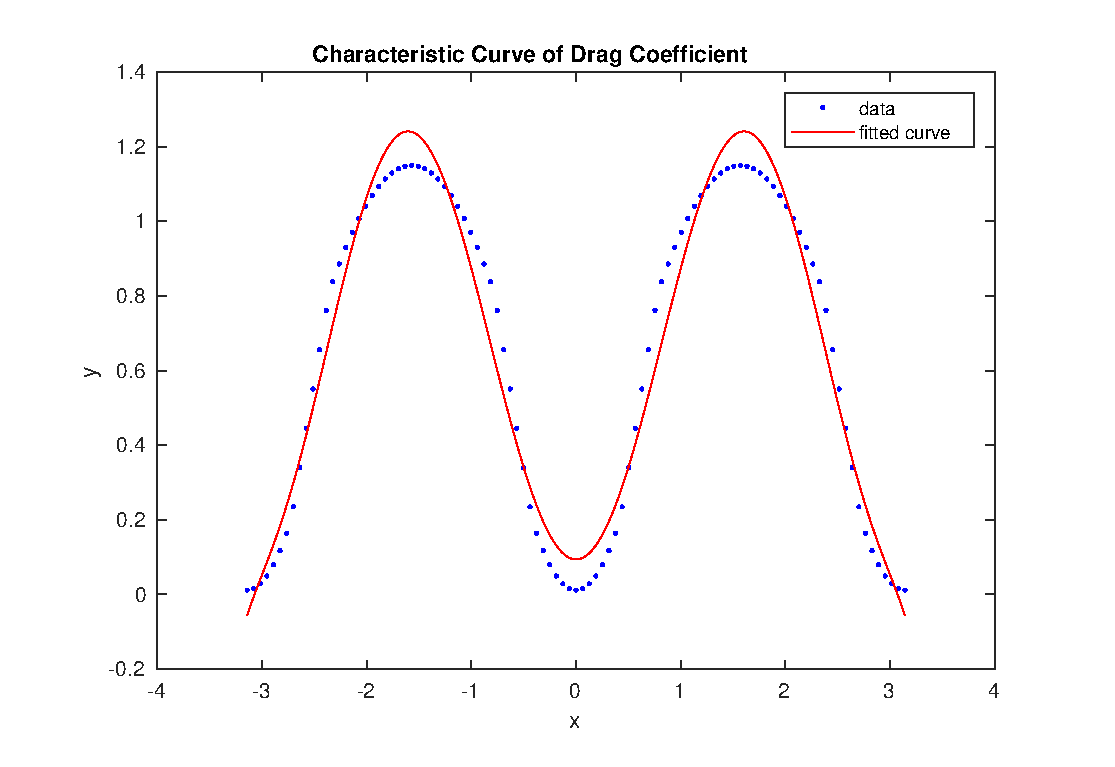
\includegraphics[width=0.75\textwidth]{dragappro.eps}
\caption{Approximation of relationship between drag coefficient $C_{D}$ and attack angle $\alpha$}	
\label{FIG:DragApprox}
\end{figure}
Strict restrictions on the fin geometric property, for instance the fins can only be mounted on the horizontal and vertical planes of the hull or they must be placed symmetrically in pairs , will bring the robot design back into the traditional way. 

A compromise can be found by means of small angle of attack assumption which is inspired by modeling methods in~\cite{FinModeling}.
\begin{figure}
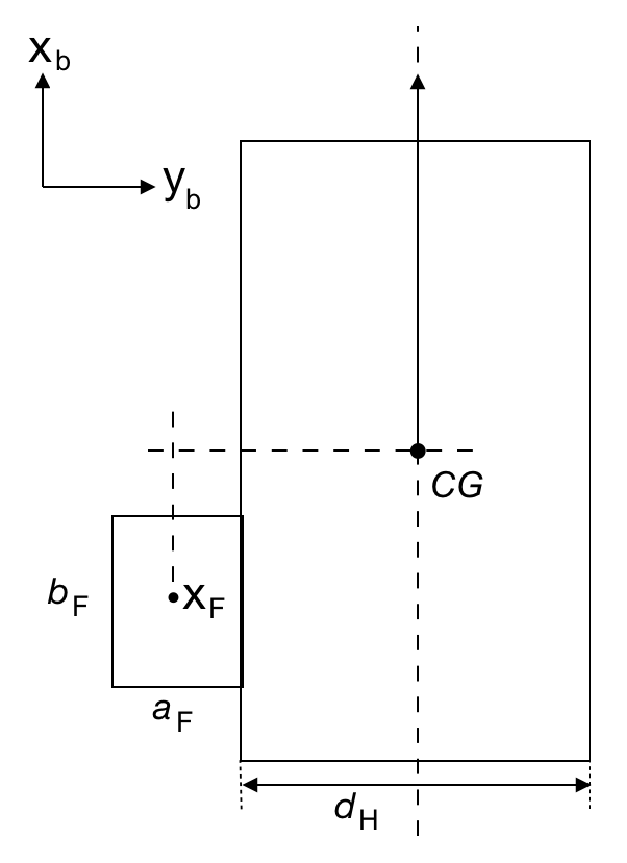
\includegraphics[width=0.4\textwidth]{FinLocation1.eps}
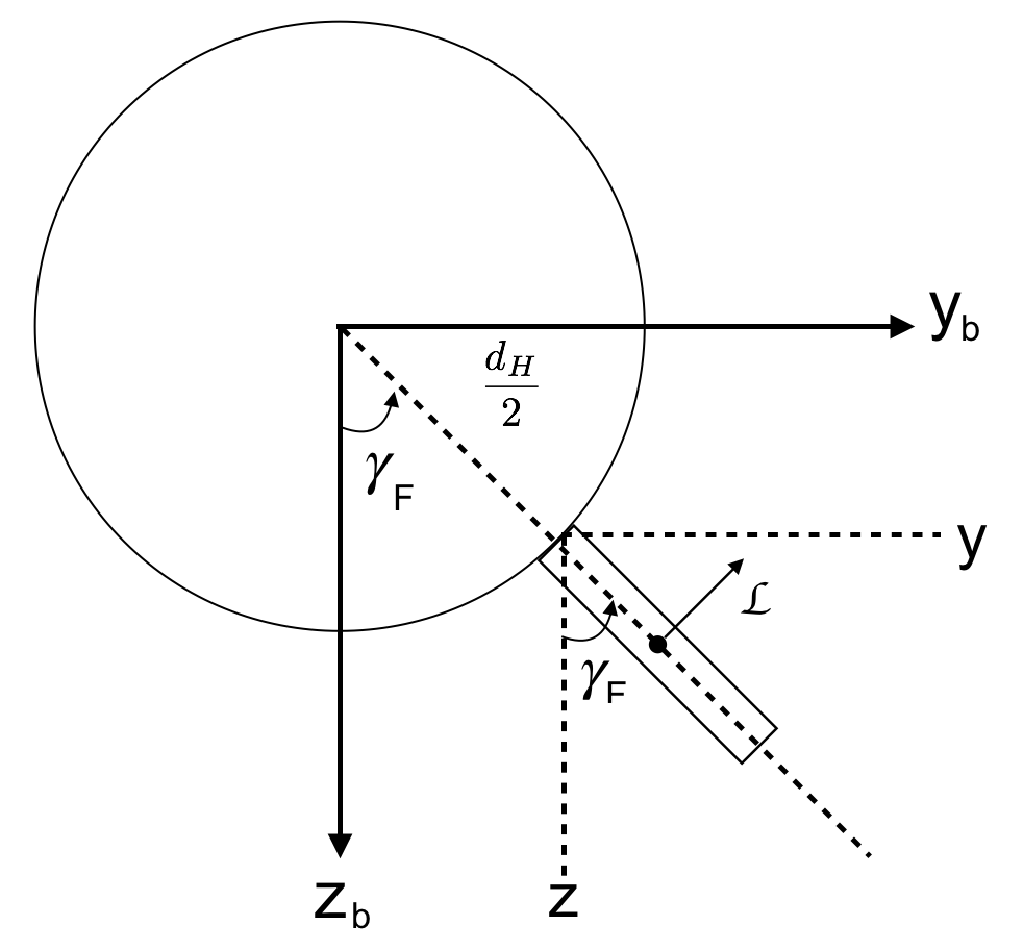
\includegraphics[width=0.4\textwidth]{FinLocation2.eps}
\caption{Definition of fin geometric parameters}	
\label{FIG:FinLocation}
\end{figure}
%\begin{figure}
%\centering
%\begin{tikzpicture}[x=1.5cm,y=1.5cm,>=latex']
%	\coordinate (O) at (-1,-1);
%	\draw[black,fill=black] (-1,-1) circle (.5ex) 
%	\coordinate (OD) at(0,-1);
%	% plot the x-axis
%	\draw [dashed] (O) -- (-1,1.5);
%	\draw [->] (O) -- (-1,1.5);
%	\draw [->] (O) -- (2,-1) node[pos=0.1] {\small ${CO}$};;
%	\draw [dashed] (O) -- (-1,-3);
%	\draw [dashed] (O) -- (-2,-1);
%	\draw (-2,1)--(0,1);
%	\draw (-2,-3)--(0,-3);
%	\draw (-2,1)--(-2,-3);
%	\draw (0,1)--(0,-3);
%	\end{tikzpicture}
%\caption{Modeling of hull as hollow cylinder} \label{fig:HullModeling}
%\end{figure}
Fins are modeled as rectangle with length $a_{F}$ and width $b_{F}$. Assume the side edge $b_{F}$ is directly attached on the hull surface. Then we represent the position and the orientation of the fins in the hull cylindrical coordinate system. As illustrated in Figure \ref{FIG:FinLocation}, $x_{F}$ is defined as the x-coordinate of fin geometric center in body frame $\lbrace b \rbrace$. We rotate the $xz$-plane of the robot body frame in the counterclockwise direction by angle $\gamma_{F}$ until the fin geometric center located in this plane. Consequently, the i-th fin geometric center vector $\vec{r}_{F,i}$ can be written as
\begin{align}
\vec{r}_{F,i}=
\begin{pmatrix}
x_{F,i} \\
0.5(d_{H}+a_{F,i})\sin(\gamma_{F,i}) \\
0.5(d_{H}+a_{F,i})\cos(\gamma_{F,i})
\end{pmatrix}
\end{align}
in body frame $\lbrace b \rbrace$.
Then we can calculate the center cross product vector as 
\begin{align}
 \vec{r}_{F,i}\times&=
 \begin{pmatrix}
   0&-\dfrac{1}{2}(d_{H}+a_{F,i})\cos(\gamma_{F,i})&\dfrac{1}{2}(d_{H}+a_{F,i})\sin(\gamma_{F,i})\\
   \dfrac{1}{2}(d_{H}+a_{F,i})\cos(\gamma_{F,i})&0&-x_{F,i}\\
   -\dfrac{1}{2}(d_{H}+a_{F,i})\sin(\gamma_{F,i})&x_{F,i}&0
 \end{pmatrix}.
\end{align}
In the following, we use $\vec{e}_{1}=[0\quad 0 \quad 1]^{T}$, $\vec{e}_{2}=[0 \quad 1\quad 0]^{T}$ and $\vec{e}_{3}=[1\quad 0 \quad 0]^{T}$ to represent unit vectors in the body frame $\lbrace b \rbrace$ and $n_{f}$ to denote the number of control fins. 
For each fin, the lift $L$ and drag $D$ of fins can be calculated as
\begin{align}
\vec{L}_{ i }(\alpha _{ i }):=a_{F,i}b_{F,i}{ C }_{ L }(\alpha _{ i })Q(U_{fin})\begin{pmatrix} 0 \\ cos({ \gamma  }_{ F,i }) \\ -sin({ \gamma  }_{ F,i }) \end{pmatrix}
\end{align}
\begin{align}
\vec{D}_{ i }(\alpha _{ i })=S{ C }_{ D }(\alpha _{ i })Q(U_{fin})\vec{e}_{1},
\end{align}
where $a_{F,i}$ and $b_{F,i}$ are the length and width of the i-th fin, respectively. $C_{L}$ is the lift coefficient of fin and $C_{D}$ is the drag coefficient. 
$Q(U_{fin})=0.5\rho U_{fin}^{2}$ is a short notation for simplicity.  $U_{fin}$ is the magnitude of fin middle point velocity vector relative to the surrounding fluid in the body frame $\lbrace b \rbrace$ and $U_{fin}=\sqrt{u_{fin}^{2}+v_{fin}^{2}+w_{fin}^{2}}$.

If the surge velocity is dominant, that is, $u$ is much bigger than $v$ and $w$, the previous formulas for calculating the lift and drag can be rewritten as
\begin{align}
\vec{L}_{ i }(\alpha _{ i }):=a_{F,i}b_{F,i}{ C }_{ L }(\alpha _{ i })Q(u_{fin})\begin{pmatrix} 0 \\ cos({ \gamma}_{ F,i}) \\ -sin({ \gamma  }_{ F,i }) \end{pmatrix}
\end{align}
\begin{align}
\vec{D}_{ i }(\alpha _{ i })=S{ C }_{ D }(\alpha _{ i })Q(u_{fin})\vec{e}_{1}.
\end{align}

It turns out the resultant force vector produced by $n_{f}$ fins can be calculated as follows: 
\begin{align}
\vec{f}_{F}(\alpha_{i} )=\begin{pmatrix} \sum _{ i=1 }^{ n_{f} }{ \vec{L}_{ i }(\alpha _{ i })^{ T }\vec{e}_{ 1 }+ } \sum _{ i=1 }^{ n_{f} }{ \vec{D}_{ i }(\alpha _{ i })^{ T }\vec{e}_{ 1 } }  \\ \sum _{ i=1 }^{ n_{f} }{\vec{L}_{ i }(\alpha _{ i })^{ T }\vec{e}_{ 2 }+ } \sum _{ i=1 }^{ n_{f} }{ \vec{D}_{ i }(\alpha _{ i })^{ T }\vec{e}_{ 2 } }  \\ \sum _{ i=1 }^{ n_{f} }{ \vec{L}_{ i }(\alpha _{ i })^{ T }\vec{e}_{ 3 }+ } \sum _{ i=1 }^{n_{f} }{ \vec{D}_{ i }(\alpha _{ i })^{ T }\vec{e}_{ 3 } }  \end{pmatrix}.
\end{align}
The resultant torque vector is calculated as:
\begin{align}
\vec{\tau} _{F}(\alpha_{i} )=\sum _{ i=1 }^{n_{f}}{ \vec{r}_{F,i} \times \vec{L}_{i}(\alpha_{i}) } +\sum _{ i=1 }^{n_{f}}{ \vec{r}_{F,i} \times \vec{D}_{i}(\alpha_{i})}.
\end{align}  
\begin{figure}
\includegraphics[width=0.8\textwidth]{SmallAOA.eps}
\caption{Small angle of attack assumption~\cite{FinModeling}}	
\label{FIG:smallAOA}
\end{figure}
For small angle of attack $\alpha$, as depicted in Figure \ref{FIG:smallAOA}, it is reasonable to approximate the lift and drag coefficients as
\begin{align}
C_{L}(\alpha_{i})=c_{L}\alpha_{i},
\end{align}    
\begin{align}
C_{D}(\alpha_{i})=c_{D}\alpha_{i}^{2},
\end{align}
where $c_{L}$, $c_{D}$ are fin-specific parameters estimated from experiments. For the following calculations, we adopt this assumption.
The drag moment of the $i$-th fin is calculated as
\begin{align}
&\vec{r}_{F,i}\times \emph{\textbf{D}}_{i}(\alpha_{i})= \nonumber \\
&\begin{pmatrix}
   0&-\dfrac{1}{2}(d_{H}+a_{F,i})\cos(\gamma_{F,i})&\dfrac{1}{2}(d_{H}+a_{F,i})\sin(\gamma_{F,i})\\
   \dfrac{1}{2}(d_{H}+a_{F,i})\cos(\gamma_{F,i})&0&-x_{F,i}\\
   -\dfrac{1}{2}(d_{H}+a_{F,i})\sin(\gamma_{F,i})&x_{F,i}&0
 \end{pmatrix} 
 \begin{pmatrix}
 c_{D}a_{F,i}b_{F,i}Q(u_{fin})\alpha_{i}^{2} \\0\\0
 \end{pmatrix} \nonumber \\
&=\begin{pmatrix}
0 \\
\dfrac{1}{2}(d_{H}+a_{F,i})\cos(\gamma_{F,i})c_{D}a_{F,i}b_{F,i}Q(u_{fin}) \\
-\dfrac{1}{2}(d_{H}+a_{F,i})\sin(\gamma_{F,i})c_{D}a_{F,i}b_{F,i}Q(u_{fin})
\end{pmatrix}
\alpha_{i}^{2}.
\end{align}
The lift moment is given by
\begin{align}
&\vec{m}_{F,i}=\vec{r}_{F,i}\times \emph{\textbf{L}}_{i}(\alpha_{i})= \nonumber \\
&\begin{pmatrix}
   0&-\dfrac{1}{2}(d_{H}+a_{F,i})\cos(\gamma_{F,i})&\dfrac{1}{2}(d_{H}+a_{F,i})\sin(\gamma_{F,i})\\
   \dfrac{1}{2}(d_{H}+a_{F,i})\cos(\gamma_{F,i})&0&-x_{F,i}\\
   -\dfrac{1}{2}(d_{H}+a_{F,i})\sin(\gamma_{F,i})&x_{F,i}&0
 \end{pmatrix} 
 \begin{pmatrix}
 0\\c_{L}a_{F,i}b_{F,i}Q(u_{fin})\cos(\gamma_{F,i})\alpha_{i}\\
c_{L}a_{F,i}b_{F,i}Q(u_{fin})\sin(\gamma_{F,i})\alpha_{i}
 \end{pmatrix} \nonumber \\
&=\begin{pmatrix}
-c_{L}a_{F}b_{F}Q(u_{fin})\dfrac{1}{2}(d_{H}+a_{F})\\
c_{L}a_{F}b_{F}Q(u_{fin})x_{F}\sin(\gamma_{F})\\
c_{L}a_{F}b_{F}Q(u_{fin})x_{F}\cos(\gamma_{F})
\end{pmatrix}
\alpha_{i}.
\end{align}
Note that the moment of fins should be calculated according the center of mass $CG$ of the whole robot, that is, $ \vec{r}_{F,i} $ here should be the vector connecting the center of fins and the center of mass $CG$. However, we assume that, for calculating the fin moments, the center of mass of the robot is the origin $CO$ of the body frame $\lbrace b \rbrace$. It means that the vector $\vec{r}_{F,i}$ denotes the position of fin geometric center in the robot body frame.

We use the lift force generated by fins as the control input and treat the drag as disturbance.

Similar to the defined mapping vector of thrusters, we also define the mapping vector for fins as follows:
\begin{align}
\emph{\textbf{B}}_{F}=
\begin{pmatrix}
0\\c_{L}a_{F}b_{F}Q(u_{fin})\cos(\gamma_{F})\\
c_{L}a_{F}b_{F}Q(u_{fin})\sin(\gamma_{F})\\
-c_{L}a_{F}b_{F}Q(u_{fin})\dfrac{1}{2}(d_{H}+a_{F})\\
c_{L}a_{F}b_{F}Q(u_{fin})x_{F}\sin(\gamma_{F})\\
c_{L}a_{F}b_{F}Q(u_{fin})x_{F}\cos(\gamma_{F})
\end{pmatrix}\in \mathbb{R}^{6}.\label{EQ:FinMappingVector}
\end{align}
The fin mapping matrix is not only geometry-dependent but also state dependent, since it contains the surge velocity term $Q(u_{fin})$. For small drift angle, the angle of attack $\alpha$ of the hydrofoils can be approximated by the mechanic
al angle of rotation of the hydrofoils~\cite{Fossen2008}. For our case, it means $\alpha=\delta_{F}$, where $\delta_{F}$ is the deflection angle of fins. Then the generalized force generated by fins can be written in the following form:
\begin{align}
\vec{\tau}_{F}=
\begin{pmatrix}
\vec{f}_{F}\\ \vec{m}_{F}
\end{pmatrix}=
\emph{\textbf{B}}_{F}\delta_{F}.
\end{align}

\section{Dynamics Construction}
The moments of inertia for each individual modules making up the robot is calculated with respect to the module's own frame, where the hull frame is usually chosen as the robot body frame $\lbrace b \rbrace$. It means, the elemental moments of inertia should be transformed to the body frame $\lbrace b \rbrace$. For each submodule whose center of gravity $ CG_{s} $ is $(x_{s}, y_{s}, z_{s})^{T}$ in body frame $\lbrace b \rbrace$, we can compute their moments of inertia in $\lbrace b \rbrace$ as follows: 
\begin{align}
I_{xx,s}^{b}=I_{xx,s}+m_{s}(y_{s}^{2}+z_{s}^{2}),\label{EQ:MomentTransfer1}
\end{align}
\begin{align}
I_{yy,s}^{b}=I_{yy,s}+m_{s}(z_{s}^{2}+x_{s}^{2}),\label{EQ:MomentTransfer2}
\end{align}
\begin{align}
I_{zz,s}^{b}=I_{zz,s}+m_{s}(x_{s}^{2}+y_{s}^{2}).\label{EQ:MomentTransfer3}
\end{align}
where $I_{xx,s}^{b}, I_{yy,s}^{b} and I_{zz,s}^{b}$ are moments of inertia with respect to the body axes $\lbrace b \rbrace$ of the component $s$. In this work, we only consider the moment of inertia of batteries, hull enclosure and the constant moment of inertia of all devices within the hull, the moments of inertia of fins, thrusters and other components are neglected.

Suppose we have totally $N$ components, then the resultant center of mass $ \vec{r}_{G} $ for the whole robot is 
\begin{align}
\vec{r}_{G}=\dfrac{\sum_{s=1}^{N}m_{s}\vec{r}_{G,s}}{\sum_{s=1}^{N}m_{s}},\label{EQ:CGAll}
\end{align} 
where $m_{s}$ is the mass of the component $s$, and $\vec{r}_{G,s}$ is the position vector of the component $s$ in the body frame $\lbrace b \rbrace$.

\section{Estimation of the Hydrodynamic Effects}
Hydrodynamic effects are the distinct feature for underwater robots. Strictly speaking, each component (hull, thrusters and fins) contributes to the hydrodynamic forces and moments. However, hydrodynamic effects depend not only on the geometric structure but also on the working condition (e.g. the inflow fluid velocity). Normally, the underwater robot dynamics is built in body frame (usually the geometric center of the hull). However, the hydrodynamic effect of each module is calculated with respect to its own geometric center. It means they should be transformed into body frame according to their positions. This transformation will make the nonlinear and strongly coupled hydrodynamic effects more complicated. Thus, the basic assumption for the estimation is that only hull contributes significantly to the hydrodynamic coefficients, while other contributions are negligible. Because we set the hull frame as the robot body frame, no transformation is needed. The hydrodynamic effects include mainly two parts: the added mass and the hydrodynamic damping. 

\subsection{Estimating the Added Mass Coefficients}
For estimating the added mass, we assume that the added mass of thrusters and fins are negligible and only the added mass of the cylindrical hull is taken into consideration. For a symmetrical cylindrical rigid body of mass $m_{H}$ with circular section of radius $r_{H}$ and length $l_{H}$, the added mass coefficients (definitions in Section~\ref{addedmassdefi}) can be derived theoretically by applying the strip theory as follows:
\begin{align}
X_{\dot{u}}=-0.1m_{H},
\end{align}
\begin{align}
Y_{\dot{v}}=-\pi\rho r_{H}^{2}l_{H},
\end{align}
\begin{align}
Z_{\dot{w}}=-\pi\rho r_{H}^{2}l_{H},
\end{align}
\begin{align}
K_{\dot{p}}=0,
\end{align}
\begin{align}
M_{\dot{q}}=-\dfrac{1}{12}\pi\rho r_{H}^{2}l_{H}^{3},
\end{align}
\begin{align}
N_{\dot{r}}=-\dfrac{1}{12}\pi\rho r_{H}^{2}l_{H}^{3}.
\end{align}
The cylindrical hull has three planes of symmetry. When the robot is completely submerged in the fluid, the added mass matrix $\emph{\textbf{M}}_{A}$ and the Coriolis matrix $\emph{\textbf{C}}_{A}$ can be calculated as follows:
\begin{align}
\emph{\textbf{M}}_{A}=diag([-X_{\dot{u}} -Y_{\dot{v}} -Z_{\dot{w}}
-K_{\dot{p}} -M_{\dot{q}} -N_{\dot{r}}]) \label{EQ:AddedMassMatrix}
\end{align}
\begin{align}
\emph{\textbf{C}}_{A}=
\begin{pmatrix}
0&0&0&0&-Z_{\dot{w}}w&Y_{\dot{v}}v\\
0&0&0&Z_{\dot{w}}w&0&-X_{\dot{u}}u\\
0&0&0&-Y_{\dot{v}}v&X_{\dot{u}}u&0\\
0&-Z_{\dot{w}}w&Y_{\dot{v}}v&0&-N_{\dot{r}}\dot{r}&M_{\dot{q}}q\\
Z_{\dot{w}}w&0&-X_{\dot{u}}u&N_{\dot{r}}r&0&-K_{\dot{p}}p\\
-Y_{\dot{v}}v&X_{\dot{u}}u&0&-M_{\dot{q}}q&K_{\dot{p}}p&0
\end{pmatrix}. \label{EQ:CoriolisMatrix}
\end{align}
\nm{$\emph{\textbf{C}}_{A}$}{Added Coriolis Matrix}

The total mass matrix is
\begin{align}
\emph{\textbf{M}}=\emph{\textbf{M}}_{RB}+\emph{\textbf{M}}_{A}.
\end{align}
Since $\emph{\textbf{M}}_{RB}\succ 0$ and $\emph{\textbf{M}}_{A}\succeq 0$, the complete robot inertia matrix is positive definite, i.e., $\emph{\textbf{M}}\succ 0$, thus $\emph{\textbf{M}}$ is invertible.  


%The vehicle is approximated as an ellipsoid characterized by the parametric representation:
% \begin{align}
% \dfrac{x^{2}}{a^{2}}+\dfrac{y^{2}}{b^{2}}+\dfrac{z^{2}}{c^{2}}=1
% \end{align} 
% where $b=c$ and $a>c$, and the eccentricity $e_{c}=1-(b/a)^{2}$. Then % the ellipsoid can be rewritten as
% \begin{align}
% \dfrac{x^{2}}{a^{2}}+\dfrac{y^{2}+z^{2}}{b^{2}}=1
% \end{align}





% Being $b=c$ and $a>c$, it can be noticed that a prolate spheroid  
% The rigid body matrix
% \begin{align}
% \emph{\textbf{M}}^{CO}_{RB} &=
% \begin{pmatrix}
% m\emph{\textbf{I}}_{3\times 3}&-m\emph{\textbf{S}}(\vec{r}_{g}^{b}) \\
% m\emph{\textbf{S}}(\vec{r}_{g}^{b})&
% \emph{\textbf{I}}_{g}-m\emph{\textbf{S}}^{2}(\vec{r}^{b}_{g})
% \end{pmatrix}
% \end{align}
% The eccentricity is defined as 
% \begin{align}
% e_{c}=1-(b/a)^{2}
% \end{align} 
% \begin{align}
% \alpha_{0}=\dfrac{2(1-e_{c}^{2})(\dfrac{1}{2}\log\left(\dfrac{1+e_{c}}{1-e_{c}}\right)-e_{c})}{e_{c}^{3}}
% \end{align}
% \begin{align}
% \beta_{0}=\dfrac{1}{e_{c}^{2}}-\dfrac{(1-e_{c}^{2})\log\left(\dfrac{1+e_{c}}{1-e_{c}}\right)}{2e_{c}^{3}}
% \end{align}
% Based on these two parameters 
% \begin{align}
% X_{\dot{u}}=-m\dfrac{\alpha_{0}}{2-\alpha_{0}}
% \end{align}
% \begin{align}
% Y_{\dot{v}}=-m\dfrac{\beta_{0}}{2-\beta_{0}}
% \end{align}
% \begin{align}
% Z_{\dot{w}}=Y_{\dot{v}}
% \end{align}
% \begin{align}
% M_{\dot{q}}=-\dfrac{m}{5}\dfrac{(b^{2}-a^{2})^{2}(\alpha_{0}-\beta_{0})}{2(b^{2}-a^{2})-(b^{2}+a^{2})(\alpha_{0}-\beta_{0})}
% \end{align}
% \begin{align}
% N_{\dot{r}}=M_{\dot{q}}
% \end{align}

\subsection{Estimating the Damping Coefficients}
The hydrodynamic damping can be modeled as:
\begin{align}
F_{H}=-\dfrac{1}{2}\rho C_{D}A_{r}|\nu|\nu, 
\end{align}
where $\rho$ is the fluid density, $C_{D}$ is the drag coefficient, $A_{r}$ the reference area, and $\nu$ is an arbitrary linear or angular velocity.
% The drag coefficient is a function of the Reynolds number $Re$, which is % defined as
% \begin{align}
% Re=\dfrac{vl}{\nu}.
% \end{align}
% where $v$ is the velocity of the fluid (SI units: $m/s$), $l$ is the % characteristic linear dimension ($m$) and $\nu$ is the kinematic viscosity of %the fluid ($m^{2}/s$). 
To estimate the drag coefficient of the robot hull, we make the following the assumptions:
\begin{enumerate}
\item The drag coefficient $C_{D}$ is dependent on the Reynolds number $Re$, the Mach number $Ma$ and the direction of the flow. Low Mach number is assumed, in this case the drag coefficient is independent of it. We also assume high speed manoeuvring where the incoming flow direction is more-or-less the same and the drag coefficient $C_{D}$ can be treated as a constant~\cite{wikiDragCoefficient}.
\item The skin friction is neglected.
\item The underwater robot is performing a non-coupled motion.
\item The quadratic damping terms are dominant.
\item The lift force of the hull is not considered.
\end{enumerate}
The damping matrix is defined as
\begin{align}
\emph{\textbf{D}}=
diag([-X_{u|u|}|u|,-Y_{v|v|}|v|,-Z_{w|w|}|w|,-K_{p|p|}|p|,-M_{q|q|}|q|,-N_{r|r|}|r|]).
\end{align}
The damping coefficient in the x-direction due to the viscous force acting on the frontal area is given as 
\begin{align}
X_{|u|u}=-\dfrac{1}{2}\rho C_{D}A_{frontal}=-\dfrac{1}{2}\rho\pi C_{D}r_{H}^{2},
\end{align}
The damping coefficients in the y and z axes due to viscous effects on the side projected areas of the hull is given as
\begin{align}
Y_{|v|v}=-\dfrac{1}{2}\rho C_{D}2r_{H}l_{H}
\end{align}
and 
\begin{align}
Z_{w|w|}=-\dfrac{1}{2}\rho C_{D}2r_{H}l_{H}
\end{align}
respectively.

%The rotation drag is neglected since for stable underwater robot motion, %angular velocities are very small. 

% The drag coefficient $ X_{u|u|}=-0.5\rho \pi a^{2}C_{d}$ and $Y_{v|v|}=Z_{w|% w|}=X_{u|u|}\dfrac{a}{b}$.

%The rigid body Coriolis Matrix can be written componentwise as follows:
%\begin{align}
%\begin{pmatrix}
%0&0&0&-m(y_{g}q+z_{g}r)
%\end{pmatrix}
%\end{align} 
%\begin{gather}\label{EQ:RigidCoriolis}
%\emph{\textbf{C}}_{RB}(\vec{\upsilon})=
%\left(
%\begin{matrix} 
%0&0&0 \\
%0&0&0 \\
%0&0&0 \\
%-m(y_{g}+z_{g}r)&m(y_{g}p+w)&m(z_{g}p-v)\\
%m(x_{g}q-w)&-m(z_{g}r+x_{g}p)&m(z_{g}q+u)\\
%m(x_{g}r+v)&m(y_{g}r-u)&-m(x_{g}p+y_{g}q)
%\end{matrix}
%\right.
% \nonumber\\
%\qquad \qquad\left. 
%\begin{matrix} {m(y_{g}q+z_{g}r)} & {-m(x_{g}q-w)} & {-m(x_{g}r+v)} \\
%-m(y_{g}p+w) & m(z_{g}r+x_{g}p) & -m(y_{g}r-u) \\
%-m(z_{g}p-v) & -m(z_{g}q+u) & m(x_{g}p+y_{g}q) \\
%0 & -I_{yz}q-I_{xz}p+I_{z}r & I_{yz}r+I_{xy}p-I_{y}q \\
%I_{yz}q+I_{xz}p-I_{z}r &0& -I_{xz}r-I_{xy}q+I_{x}p \\
%-I_{yz}r-I_{xy}p+I_{y}q&I_{xz}r+I_{xy}q-I_{x}p &0 
%\end{matrix}
%\right)
%\end{gather}
The hull has no contribution to the roll moment, hence 
\begin{align}
K_{p|p|}=0.
\end{align}
   
The drag force due to pitch motion is given as
\begin{align}
M_{q|q|}q|q|=-\dfrac{1}{2}\rho w|w| \int^{l_{H}/2}_{-l_{H}/2}C_{D}~2r~dx~x
\end{align}
For small angular motions, $w\approx q x$. Thus, the pitch damping coefficient is given by
\begin{align}
M_{q|q|}=-\dfrac{1}{12}\rho C_{D} r_{H}l_{H}^{4}
\end{align}
Similarly, the horizontal drag forces contribute the yaw drag, whose coefficient is same as the pitch drag:
\begin{align}
N_{r|r|}=-\dfrac{1}{12}\rho C_{D} r_{H}l_{H}^{4}
\end{align}
The details for derivation of these parameters can be found in~\cite{Sia1999}, it also includes the drag caused by thrusters and struct linking hull and thruster which could be for future work. With help of two geometric parameters $l_{H}$ and $r_{H}$, the hydrodynamic terms in the robot dynamic equation including $\emph{\textbf{M}}_{A}$, $\emph{\textbf{C}}_{A}$ and $\emph{\textbf{D}}$ can be computed.

To sum up, in this chapter we model the robot hull, batteries, fins as simple geometric shapes determined by several geometric parameters. In addition, for thrusters we only pay attention on their positions, motor orientations and spin directions regardless of their shapes. By means of this modeling method, we are able to construct a customizable robot dynamics parametrized with these geometric parameters. They will be chosen as decision variables for the robot geometry optimization so that the current dynamics can be computed at each optimization iteration. 
%____________________________________________________